\documentclass{article}
\usepackage[utf8]{inputenc}
\usepackage{polski}
\usepackage{geometry}
\usepackage{pdfpages}
\usepackage{pdfpages}
\usepackage{listings}
\usepackage{listingsutf8}
\usepackage{multirow}
\usepackage{siunitx}
\usepackage{multirow}
\usepackage{booktabs}
\usepackage{tabularx}
\usepackage{placeins}
\usepackage{pdflscape}
\usepackage{graphicx}
\usepackage{subfig}
\usepackage{hyperref}
\usepackage{amsmath}
\usepackage{colortbl}

\geometry{
a4paper,
total={170mm,257mm},
left=20mm,
top=20mm
}
\newcolumntype{Y}{>{\centering\arraybackslash}X}
% \renewcommand\thesection{}
\lstset{%
literate=%
 {ą}{{\k{a}}}1
 {ę}{{\k{e}}}1
 {Ą}{{\k{A}}}1
 {Ę}{{\k{E}}}1
 {ś}{{\'{s}}}1
 {Ś}{{\'{S}}}1
 {ź}{{\'{z}}}1
 {Ź}{{\'{Z}}}1
 {ń}{{\'{n}}}1
 {Ń}{{\'{N}}}1
 {ć}{{\'{c}}}1
 {Ć}{{\'{C}}}1
 {ó}{{\'{o}}}1
 {Ó}{{\'{O}}}1
 {ż}{{\.{z}}}1
 {Ż}{{\.{Z}}}1
 {ł}{{\l{}}}1
 {Ł}{{\l{}}}1
}

\title{Metody Programowania Równoległego\\ Map Reduce}
\author{Maciej Trątnowiecki}
\date{AGH, Semestr Letni, 2022}

\begin{document}
    \maketitle
    \lstset{ 
      backgroundcolor=\color{white},   % choose the background color; you must add \usepackage{color} or \usepackage{xcolor}; should come as last argument
      basicstyle=\footnotesize,        % the size of the fonts that are used for the code
      breakatwhitespace=false,         % sets if automatic breaks should only happen at whitespace
      breaklines=true,                 % sets automatic line breaking
      captionpos=b,                    % sets the caption-position to bottom
      commentstyle=\color{mygreen},    % comment style
      deletekeywords={...},            % if you want to delete keywords from the given language
      escapeinside={\%*}{*)},          % if you want to add LaTeX within your code
      %extendedchars=true,              % lets you use non-ASCII characters; for 8-bits encodings only, does not work with UTF-8
      firstnumber=1000,                % start line enumeration with line 1000
      frame=single,	                   % adds a frame around the code
      keepspaces=true,                 % keeps spaces in text, useful for keeping indentation of code (possibly needs columns=flexible)
      keywordstyle=\color{blue},       % keyword style
      language=Octave,                 % the language of the code
      morekeywords={*,...},            % if you want to add more keywords to the set
      numbers=left,                    % where to put the line-numbers; possible values are (none, left, right)
      numbersep=5pt,                   % how far the line-numbers are from the code
      numberstyle=\tiny\color{mygray}, % the style that is used for the line-numbers
      rulecolor=\color{black},         % if not set, the frame-color may be changed on line-breaks within not-black text (e.g. comments (green here))
      showspaces=false,                % show spaces everywhere adding particular underscores; it overrides 'showstringspaces'
      showstringspaces=false,          % underline spaces within strings only
      showtabs=false,                  % show tabs within strings adding particular underscores
      stepnumber=2,                    % the step between two line-numbers. If it's 1, each line will be numbered
      stringstyle=\color{mymauve},     % string literal style
      tabsize=2,	                   % sets default tabsize to 2 spaces
      title=\lstname                   % show the filename of files included with \lstinputlisting; also try caption instead of title
    }
        % \lstinputlisting[language=python]{../ex1/ping_pong.py}

        % \begin{center}
        %     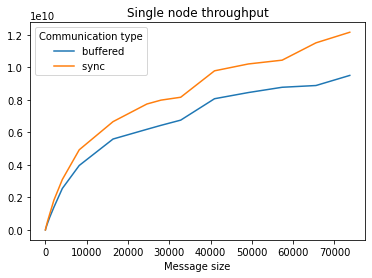
\includegraphics[width=13cm]{report1/images/ex1_single_node.png}
        %     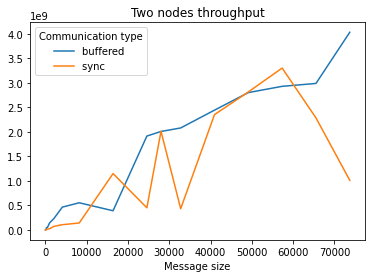
\includegraphics[width=13cm]{report1/images/ex1_two_nodes.png}
        % \end{center}

        % \begin{center}
        %     \begin{table}[ht]
        %         \centering
        %         \begin{tabular}{|c|c|c|}
        %             \hline
        %             Rodzaj komunikacji  & Typ wiadomości & Przepustowość [Mbit/s]\\
        %             \specialrule{1pt}{1pt}{1pt}
        %             Jeden węzeł & buforowana & 1.105\\
        %             \hline
        %         \end{tabular}
        %         \caption{Opóźnienie w przesłaniu wiadomości.}
        %     \label{tab:my_label}
        %     \end{table}
        % \end{center}
        
        
    \section{Sformułowanie problemu}
    W ramach zadania przygotowałem sekwencyjną implementację algorytmu zliczającego wystąpienia słów w tekście. Następnie wykonałem pomiary czasu wykonania zarówno wspominanej wersji sekwencyjnej jaki i przygotowanej w ramach laboratorium implementacji dla frameworka hadoop. 
    
    \section{Środowisko uruchomieniowe}
    Wersję równoległą uruchamiałem w środowisku \textit{EMR} z chmury \textit{AWS}. Wersję sekwencyjną na maszynie wirtualnej z usługi \textit{EC2} w tej samej chmurze. 
        \begin{center}
            \begin{table}[ht]
                \centering
                \begin{tabular}{|c|c|c|c|c|}
                    \hline
                    Usługa  & Nazwa instancji & Ilość Węzłów & Ilość rdzeni na węzeł & Sumaryczna ilość rdzeni\\
                    \specialrule{1pt}{1pt}{1pt}
                    EC2 & m4.large & 1 & 2 & 2\\
                    EMR & m4.large & 12 & 2 & 24\\
                    EMR & m4.xlarge & 6 & 4 & 24\\
                    \hline
                \end{tabular}
                \caption{Konfiguracja instancji.}
            \label{tab:my_label}
            \end{table}
        \end{center}
    Zauważyć należy, że \textit{m4.large} i \textit{m4.xlarge} oferują identyczne procesory wirtualne, lecz różnią się ich ilością i konfiguracją. 
    
    \section{Implementacja sekwencyjna}
    Implementację sekwencyjną algorytmu wykonałem w języku \textit{C++}. Wczytuje ona dane wyjściowe z jednego pliku, a wyniki zapisuje w drugim. Kod źródłowy załączam poniżej. 
    \lstinputlisting[language=cpp]{../counter.cpp}
    
    \section{Pomiary}
    Przygotowałem pomiary czasu wykonania algorytmu dla danych wejściowych rozmiaru kolejno \textit{1GB}, \textit{5GB} i \textit{10GB}. Każdy z pomiarów uruchomiłem dziesięciokrotnie dla każdej z konfiguracji sprzętowych opisanych w tabeli powyżej. Wyniki przedstawiłem na wykresach. 
    \begin{figure}[h!]
        \centering
        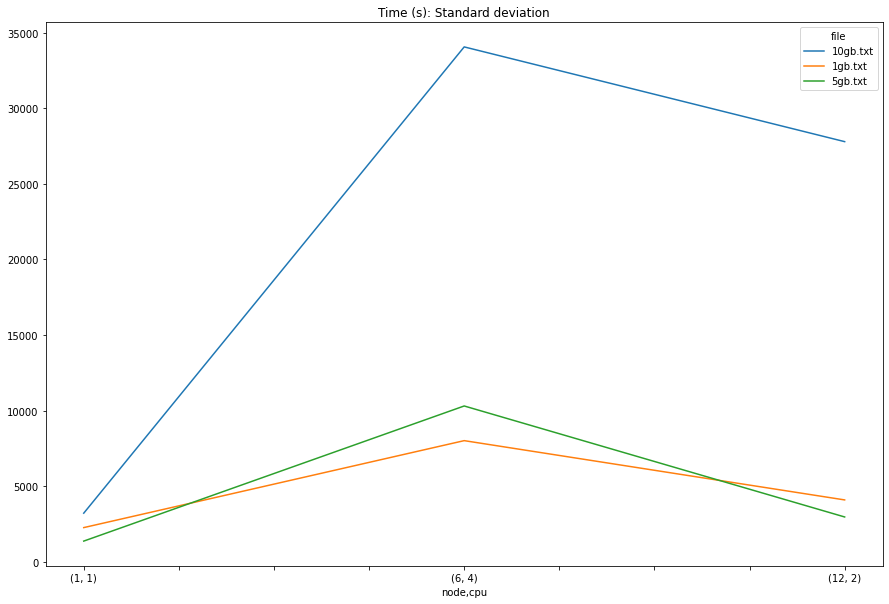
\includegraphics[width=15cm]{ex4/report/time_std.png}
        \caption{Odchylenie standardowe pomiarów}
    \end{figure}
    \begin{figure}[h!]
        \centering
        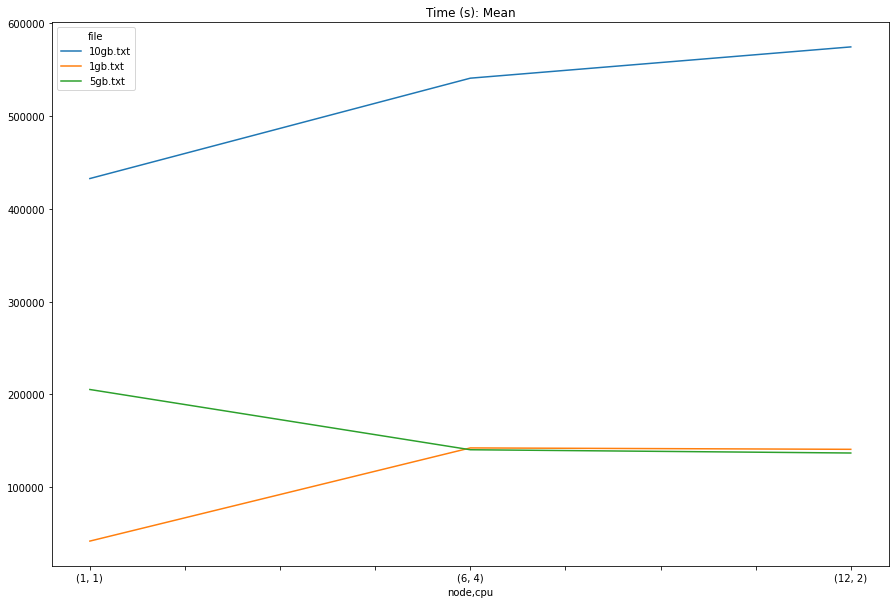
\includegraphics[width=15cm]{ex4/report/time_mean.png}
        \caption{Średni czas wykonania programu w \textit{ms}}
    \end{figure}
    
    \newpage
    Następnie obliczyłem przyśpieszenie programu dla kolejnych konfiguracji sprzętowych, w oparciu o średni czas wykonania programu. 
    \begin{figure}[h!]
        \centering
        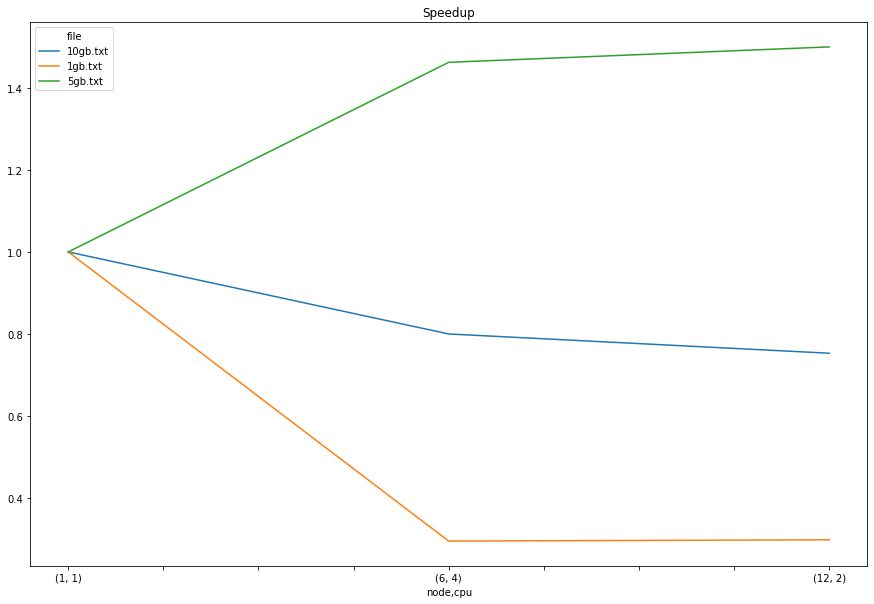
\includegraphics[width=13cm]{ex4/report/speedup.png}
        \caption{Przyśpieszenie}
    \end{figure}

    \section{Wnioski}
    Łatwo zauważyć, że implementacja sekwencyjna paradoksalnie okazała się szybsza od implementacji równoległej dla wszystkich konfiguracji i rozmiarów plików, za wyjątkiem pliku o rozmiarze \textit{5GB}.\\
    
    Potencjalnie wynika to z faktu, że wykorzystałem dobrze zoptymalizowaną, kompilowaną implementację sekwencyjną, która naturalnie lepiej radzi sobie z przetwarzaniem dużych rozmiarów danych niż te wykonane w językach interpretowanych. W przypadku plików odpowiednio małych (w moim przypadku \textit{1GB}), ta specyfika jest wystarczająca do otrzymania lepszych wyników. W przypadku plików odpowiednio dużych (w moim przypadku \textit{10GB}), występujące obciążenia komunikacyjne mogą potencjalnie zajmować więcej czasu niż samo wykonanie obliczeń. W przypadku średnim natomiast lepsza skalowalność rozwiązania równoległego pozwoliła na otrzymanie lepszych wyników i krótszych czasów wykonania niż sekwencyjna. Potencjalnie moglibyśmy otrzymać lepsze wyniki, dla największego pliku, mając dostęp do mocniejszych węzłów obliczeniowych, a przez to obniżając narzuty wynikające z komunikacji pomiędzy węzłami. \\
    
    Warto zauważyć, że generalnie konfiguracja sprzętowa o mniejszej ilości mocniejszych węzłów obliczeniowych skutkuje niższymi czasami wykonania niż konfiguracje o większej liczbie słabszych węzłów, pomimo że suma rdzeni obliczeniowych jest w obu przypadkach taka sama. Jest to efekt oczekiwany, ze względu na występujące w nich mniejsze obciążenie wynikające z komunikacji pomiędzy węzłami.\\
    
    Dla tak zdefiniowanego problemu obliczeniowego nie da się wskazać wartości metryki \textit{COST} na podstawie danych zebranych w ramach zadania. Dla dwóch z rozmiarów plików wejściowych implementacja równoległa osiągnęła gorsze niż sekwencyjna czasy wykonania, co wyklucza wskazanie konkretnej wartości metryki. W przypadku średniego rozmiaru pliku możemy wskazać, że wartość metryki jest mniejsza niż \textit{24} rdzenie, choć jej konkretna wartość nie wynika z wykresu (potencjalnie mniejsza ilość rdzeni pozwoliłaby na przecięcie progu w postaci czasu sekwencyjnego wykonania obliczeń.

\end{document}
